\chapter{绪论}\label{chap:kondo}

\section{冷原子概述}


\section{冷原子基本实验技术}

\section{少体严格解}\label{sec:fewbody}

伴随着冷原子平台实验技术的进步,各个凝聚态研究领域掀起了不同程度的热潮。其中低维少体物理的研究领域有了较大进展。得益于实验中少量原子体系的
制备、调控与测量,低维少体物理中很多概念诸如少体束缚态、玻色子费米化等理论概念不断地在冷原子实验中被观测到,并进而引发了冷原子特性平台下相关少体物理的理论研究。在本章中我们简要地选取几个一维冷原子少体领域的实验与理论研究进展,以期为接下来的研究提供启发。实际的冷原子少体体系中几个原子被束缚在势阱中,因此我们的内容也主要限制在抛物线型束缚势阱中的一维少体。由于原子间全同性原理,我们将围绕玻色少体体系与费米少体体系分别展开。服从两种统计的少体体系原子之间的相互作用均可以调节,从极弱到极强。从吸引到排斥,带来少体体系丰富的物理相图。


少体物理之所以重要很大原因在于存在严格解。对于量子力学发展初期的谐振子严格解与氢原子模型严格解的理解,几乎构成了我们理解量子力学的基石。进一步地,1998年T. Busch给出了又一个少体体系严格解:任意维度下两个全同玻色子在谐振子势场下的能谱。以一维为例,系统的哈密顿量可以写为:
\begin{equation}
\hat{\mathcal{H}}=-\frac{\hbar}{2 m}\left(\frac{\partial^{2}}{\partial x^{2}}+\frac{\partial^{2}}{\partial y^{2}}\right)+\frac{m \omega^{2}}{2}\left(x^{2}+y^{2}\right)+g \delta(x-y)
\end{equation}
其中$m$为全同玻色子的质量,$\omega$为谐振子势场的特征频率。引入一维散射长度$g= -\frac{2\hbar^2}{m}\cdot\frac{1}{a}$并分离质心运动与相对运动$R = \frac{x+y}{\sqrt{2}}, \quad X = \frac{x-y}{\sqrt{2}}$
得到$\hat{\mathcal{H} } = \hat{\mathcal{H}}_R+ \hat{\mathcal{H}}_X$:
\begin{equation}
\begin{aligned}
&\mathcal{H}_{R}=-\frac{1}{2} \frac{\mathrm{d}^{2}}{\mathrm{~d} R^{2}}+\frac{1}{2} R^{2} \\
&\mathcal{H}_{X}=-\frac{1}{2} \frac{\mathrm{d}^{2}}{\mathrm{~d} X^{2}}+\frac{1}{2} X^{2}+\frac{g}{\sqrt{2}} \delta(X)
\end{aligned}
\end{equation}
$mathcal{H}_{X}$在谐振子基矢下对角化,其中奇宇称的谐振子能级不受影响仍为$(2n+\frac{1}{2})\hbar\omega$。偶宇称的本征解能量$E_n$满足自洽方程为:
\begin{equation}
	-g \Gamma\left(\frac{1-2 E_{k}}{4}\right)=2 \sqrt{2} \Gamma\left(\frac{3-2 E_{k}}{4}\right)
\end{equation}
相应的本征波函数为:
\begin{equation}
	\Psi_{k}(X)=N_{k} \mathrm{e}^{-X^{2} / 2} \mathrm{U}\left(\frac{1-2 E_{k}}{4}, \frac{1}{2}, X^{2}\right)
\end{equation}
当相互作用$g\to\infty$时候:
\begin{equation}
\begin{split}
	E_k &\to (2k+1+1/2)\hbar\omega\\
	\Psi_{k}(X) &\to \psi_{2k+1}(X)\cdot sign(X)\\
\end{split}
\end{equation}
其中$\psi_{2k+1}(X)$为谐振子第$2k+1$个本征波函数。整个系统的能谱如图~\ref{chap1fig1}~所示
\begin{figure}[!htbp]
    \centering
    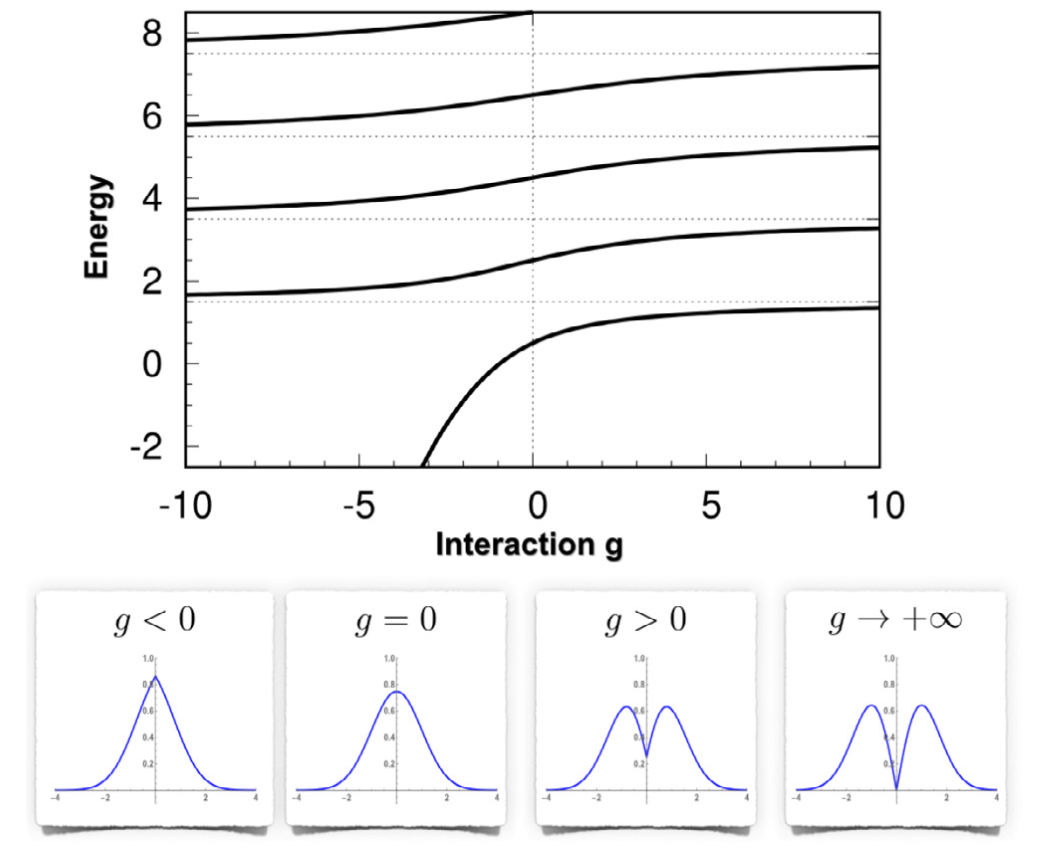
\includegraphics[width=0.6\textwidth]{chap1fig1.png}
    \bicaption{摘自1D少体势阱}{Reprinted from 1Dfewtrap}
    \label{chap1fig1}
\end{figure}
其中当$g\to-\infty$时候,基态能量渐近行为是$E_g\to-\frac{g^2}{2}$,称为lower branch。其余的随着$g\to\infty$本征能量饱和在奇数谐振子能量的态称为upper branch。这个少体体系的严格解在后续的实验与理论发展中起了很重要的做用。{\color{red}后续有一些进一步的推广。}


\subsection{玻色少体体系}
在玻色子少体体系中,无相互作用极限下体系处于BEC极限。所有的玻色子位于体系的基态。而一旦打开玻色子之间相互作用之后,新奇的物理现象就出现了。在这里我们主要讨论T-G气体与费米化。


\subsection{费米少体体系}


有了上面介绍的量子少体研究进展,将有几个可扩展的方向,比如改变相互作用,dipole、库伦、以及自旋交换相互作用,这将是下一章节介绍的。

\section{自旋交换相互作用}\label{sec:spin-exchange}
在超冷原子实验平台中,原子作为一个整体

\section{极化子理论与实验}


